% !TEX root =  ../Dissertation.tex

\chapter{Design}

The design section describes the systems needed to extract the dependency
graphs and analyse them. Agda Tree analyses two dependencies graphs, one for
modules and another for definitions. The module dependency graph can be
generated with Agda but for the definition dependency graph is created
manually.

Agda Comp is a simpler tool, as the complexity comes from testing the different
compilation strategies. It creates the module dependency graph, apply the
given strategy using the parameters provided by the user, and compile with the
order. 

\pagebreak

\section{Agda Tree}

Agda Tree is a command line interface that lets the user interact with the
module and definition graphs. The first command designed is how the both
dependency graphs are created. \cref{fig:Agda Create Tree Diagram} illustrates
how the user will interact with the CLI to create the graphs. The user provides
the Agda file that they want to analyse, normally this would be the entire
everything index file. The everything index file is the file that imports all
the modules in a project. This is standard in Agda, as this is the only way to
type-check the whole project. Depending on the Agda project, this file will be
generated automatically or by the project maintainers.
\begin{figure}[H]
    \centering
    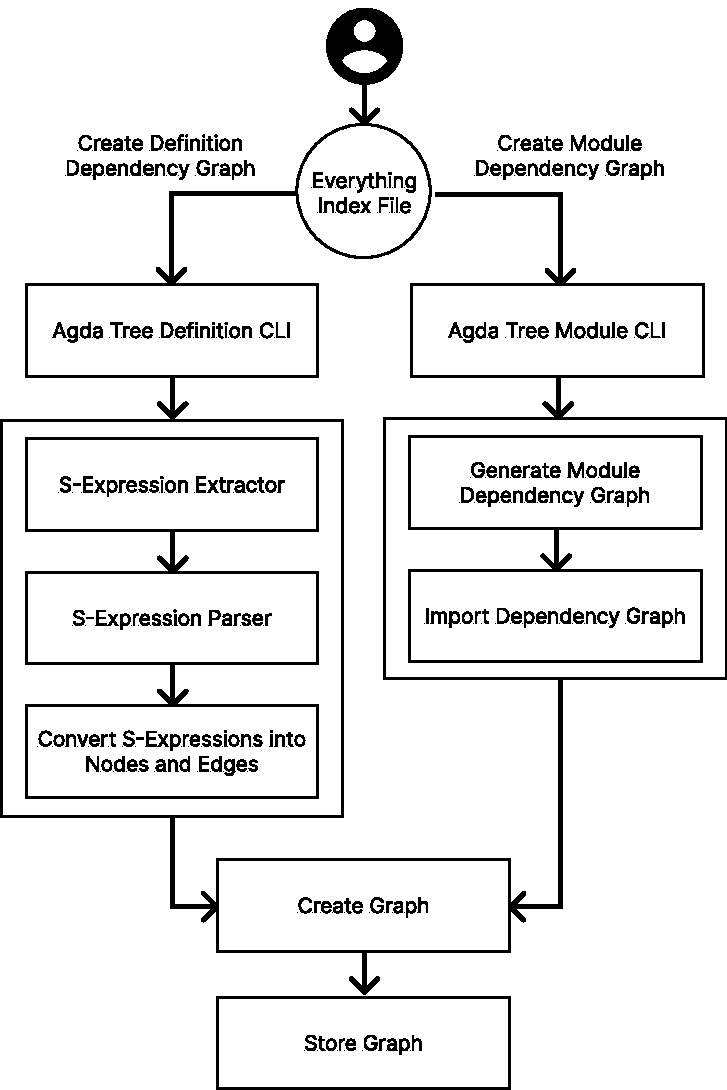
\includegraphics[scale=0.8]{Agda Create Tree.pdf}
    \caption{Agda Create Tree Diagram}
    \label{fig:Agda Create Tree Diagram}
\end{figure} 

\pagebreak

\cref{fig:Agda Tree Class Diagram} is a Class Diagram, showing the classes and
methods to operate the command line. The program starts with the command line's
entry point, that will parse the input by the user and delegate the query to
the respective dependency graph. Each dependency graph allows for a different
set of queries. These queries can be found in \cref{tbl:Definition Graph
Queries} for the definition graph and in \cref{tbl:Module Graph Queries} for
the module graph.

The definition graph creation depends on the s-expression extractor and parser.
They read the Agda projects and convert the data found into the dependency
graph.

\begin{figure}[H]
    \centering
    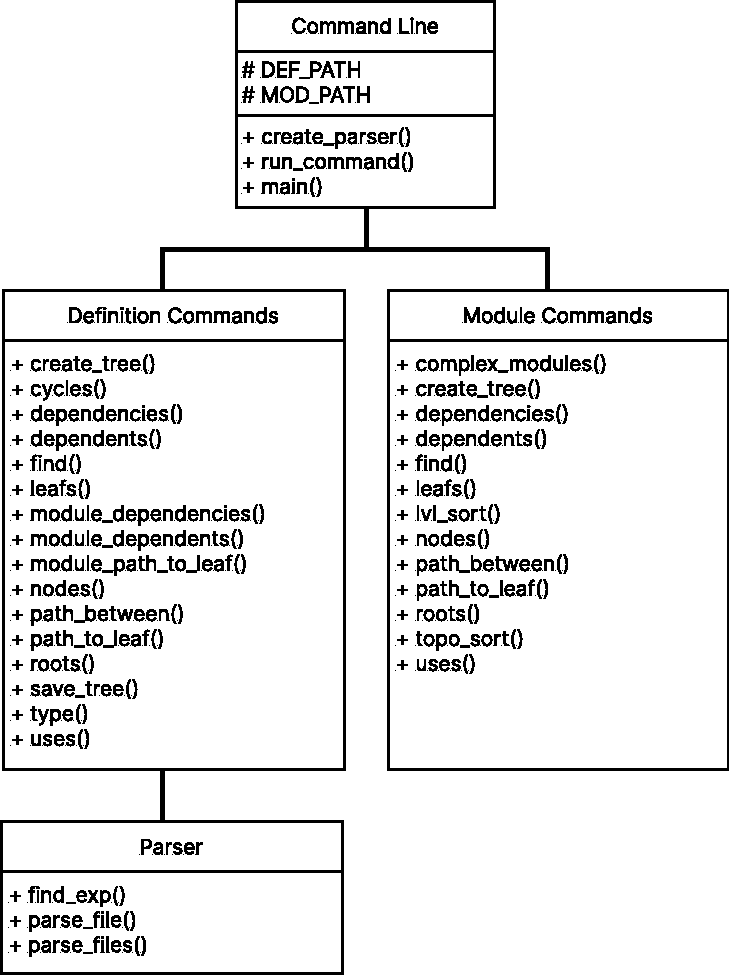
\includegraphics[scale=0.8]{Agda Tree Class Diagram.pdf}
    \caption{Agda Tree Class Diagram}
    \label{fig:Agda Tree Class Diagram}
\end{figure} 
    
\pagebreak

\cref{fig:Agda Tree Query Diagram} shows how is split CLI into two, depending
on what dependency graph is being queried. When the user makes a query, they
will select the dependency graph and the respective queries will perform that
query. The output will be displayed in stdout, which can be used with other
operations like piping and xargs.

\begin{figure}[H]
    \centering
    \includegraphics[scale=0.8]{Agda Make Query.pdf}
    \caption{Agda Tree Query Diagram}
    \label{fig:Agda Tree Query Diagram}
\end{figure} 

\pagebreak 


\section{Agda Comp}

\cref{fig:Agda Comp Diagram} demonstrates how the user will interact with
the Agda Comp tool. The user provides the module that to be compiled, next to some
parameters defining the amount of cores used in the parallelization and the
compilation strategy to use.
\begin{figure}[H]
    \centering 
    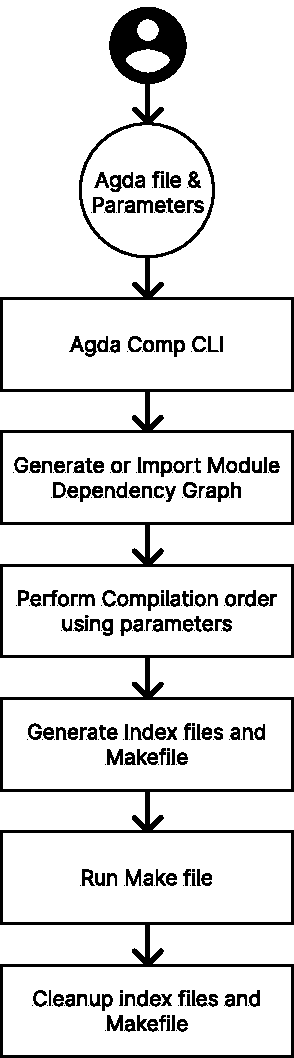
\includegraphics[scale=0.8]{Agda Comp.pdf}
    \caption{Agda Comp Diagram}
    \label{fig:Agda Comp Diagram}
\end{figure} 

\pagebreak
\subsection{Level Strategy} \label{sub:design level strategy}

The level strategy sorts the modules into levels, where leaf nodes with no
children are at level \(0\). Level \(1\) contains all the modules which only depend on
modules at level \(0\). Level \(n\) contains all the modules that depend on levels \(n
- 1\) or below. In other words, the level of a module is its maximum distance
from a leaf module. This algorithm can be visualized with the \cref{subfig: lvl strat}.
\begin{figure}[H]
  \begin{subfigure}[t]{0.45\textwidth}
    \centering
    \includegraphics[scale=0.9]{lvl_graph.pdf}
    \caption{Example dependency graph}
    \label{fig:example lvl dep graph}
  \end{subfigure} \hfill
  \begin{subfigure}[t]{0.45\textwidth}
    \centering
    \includegraphics[scale=0.9]{lvl_sort.pdf}
    \caption{Example dependency graph sorted by levels where green means level
    0, red level 1 and blue level 2}
    \label{fig:example lvl sort}
  \end{subfigure}
  \caption{Level Strategy Example}
  \label{subfig: lvl strat}
\end{figure}

This sorting has the property that each level only depends on the levels
below it, meaning if the below modules were already compiled the modules at the
current level could all be compiled in parallel. The level strategy is to sort
the modules into levels, then compile each level linearly and the modules at
each level are compiled concurrently. This strategy also compiles every module
in the graph as the sorting keeps all the modules in the dependency graph and
the level strategy compiles every level. Therefore, this algorithm is both safe
and correct.

The advantage of this solution is that it can be quickly generated,
where each module will take the maximum of the recursive call to its children
and add one the maximum of the children's level. The disadvantage is that if a
level has a small amount of modules there isn't an opportunity to
parallelize the type checking. Also, there could be two modules that each
depend  on 20 distinct modules that could be compiled in parallel that could
lead to massive savings. Instead, this method would compile the 40 combined
dependencies in previous levels, then compile the two modules in parallel. This
becomes significant during implementation \cref{sub:imp lvl strategy}, as there
is an overhead to parallelization which is exacerbated when compiling a small
collection of modules.


% \begin{itemize}
% \item What level ssortin is, connection to topo sort 
% \item Image of what the level means 
% \item How this is safe and correct from module dependency graph 
% \item How this finds parallel moduels
% \end{itemize}


\pagebreak
\subsection{Level Disjoint Strategy} \label{sub:design disjoint strategy}

The level disjoint strategy targets the weakness of the level sort strategy. It
aims to find the largest modules that can be compiled in parallel, the largest
module being one with many dependencies. If such modules are found, then they
are compiled in parallel, otherwise the leaf modules are compiled and tries
finding large modules again. Note that once a module is compiled, it is no
longer a dependency of future modules. This process is visualized below on
\cref{subfig:disj strat}.
\begin{figure}[H]
  \begin{subfigure}[t]{0.5\textwidth}
    \centering
    \includegraphics[scale=0.9]{disj_graph.pdf}
    \caption{Example dependency graph}
    \label{fig:example disj dep graph}
  \end{subfigure} \hfill
  \begin{subfigure}[t]{0.40\textwidth}
    \centering
    \includegraphics[scale=0.9]{disj_strat.pdf}
    \caption{Example dependency graph sorted where the leafs were removed,
    creating two modules that can be compiled in parallel. }
    \label{fig:example disj strat}
  \end{subfigure}
  \caption{Level Disjoint Example}
  \label{subfig:disj strat}
\end{figure}

This strategy ensures that at each step the amount of modules to compile is
reduced. The strategy only compiles two modules in parallel if their
dependencies are disjoint, if such modules aren't found then the leafs are
compiled which don't have any dependencies. Therefore, this strategy is both
safe and correct, as it doesn't compile conflicting modules and compiles all
modules in a project.

The advantage of this approach is that it manages the overhead of
parallelization, instead of compiling a couple of individual modules at a time
it can compile modules with multiple dependencies such that Agda doesn't have
to loading interface files as often as explained in the implementation
\cref{sub:imp disj strategy}. The disadvantage is that finding these disjoint
modules is difficult, projects  have hundreds of modules and finding multiple
modules that don't share dependency can't be done through brute force. Each
Agda project also has different structures with Agda-unimath
\cite{agda-unimath} having smaller independent modules while TypeTopology
\cite{type-topology} has bigger dependent modules that make finding distinct
module more difficult. A greedy approach has to be taken, which doesn't
guarantee the optimal solution.

% \begin{itemize}
% \item What level disjoint does
% \item Image of what it attemps to do
% \item How this is safe and correct from module dependency graph 
% \item How this finds parallel moduels 
% \item the greedy algorithm to find disjoint modules
% \end{itemize}


\pagebreak

\section{Conclusion}

The diagram in \cref{fig:Agda Tree Class Diagram} show how the structure of the
program. \cref{fig:Agda Create Tree Diagram} and \cref{fig:Agda Tree Query Diagram} also shows how the dependency graphs will be created and how the user
will interact with CLI. This structure is important to ensure that the
CLI can handle all the requirements and gives the project a solid foundation to
refer back to. 

The functionality of Agda Comp is modelled in Figure \cref{fig:Agda Comp Diagram}, this structure allows the user to select what compilation strategy to
use and how many cores the compilation can use. Agda Comp is lets the user to
easily apply the compilation strategies which are modelled in \cref{sub:design level strategy} and in \cref{sub:design disjoint strategy}, then are
implemented in \cref{ch:implementation}.

% Communicating how you think about the composition of your system and how it
% works. You might detail the ways in which the overall system will be broken
% down into subsystems. Detail should then be provided on the design of each of
% these subsystems.
%
% \begin{itemize} \item A system that turns agda into s-expressions \item A
% system that reads s-expressions and turns it into a graph \item A system that
% queries that graph \item A way to store the graph for future use
% \end{itemize}

